% Generated by TikzMakie.jl. Requires \usepackage{tikz} (and graphicx if images are used).
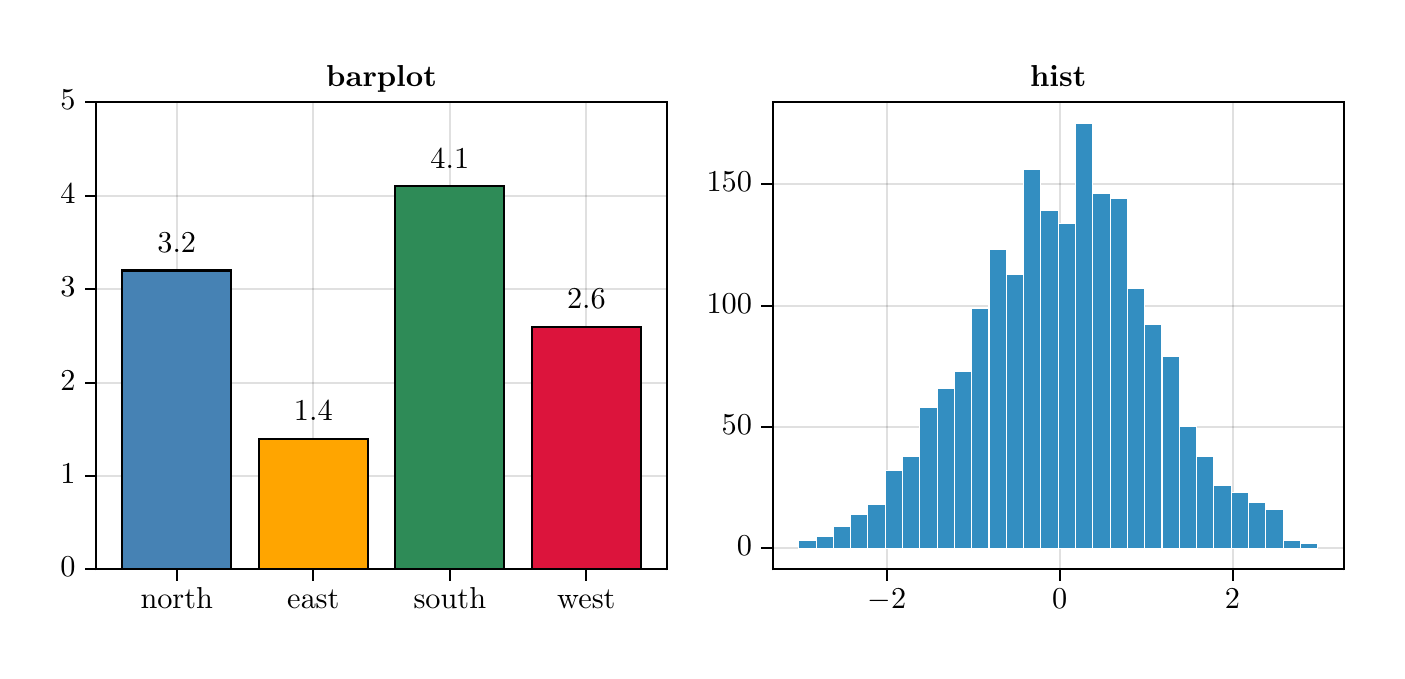
\begin{tikzpicture}[x=0.75pt, y=0.75pt, mknode/.style={inner sep=0pt, outer sep=0pt, execute at begin node={\vphantom{(}}, font=\fontsize{10.5}{12.6}\selectfont}, mkimg/.style={inner sep=0pt, outer sep=0pt}]
\definecolor{mkc1}{RGB}{70,130,180}
\definecolor{mkc2}{RGB}{255,165,0}
\definecolor{mkc3}{RGB}{46,139,87}
\definecolor{mkc4}{RGB}{220,20,60}
\definecolor{mkc5}{RGB}{51,142,193}
\path[use as bounding box] (0,0) rectangle (650,300);
\path[fill=white] (33,39) -- (308,39) -- (308,264) -- (33,264) -- cycle;
\path[fill=white] (359,39) -- (634,39) -- (634,264) -- (359,264) -- cycle;
\draw[draw=black, line width=0.75pt, draw opacity=0.12]
  (71.82,39) -- (71.82,264)
  (137.61,39) -- (137.61,264)
  (203.39,39) -- (203.39,264)
  (269.18,39) -- (269.18,264);
\draw[draw=black, line width=0.75pt, draw opacity=0.12]
  (33,39) -- (308,39)
  (33,84) -- (308,84)
  (33,129) -- (308,129)
  (33,174) -- (308,174)
  (33,219) -- (308,219)
  (33,264) -- (308,264);
\draw[draw=black, line width=0.75pt, draw opacity=0.12]
  (414.03,39) -- (414.03,264)
  (497.27,39) -- (497.27,264)
  (580.5,39) -- (580.5,264);
\draw[draw=black, line width=0.75pt, draw opacity=0.12]
  (359,49.23) -- (634,49.23)
  (359,107.67) -- (634,107.67)
  (359,166.11) -- (634,166.11)
  (359,224.55) -- (634,224.55);
\node[mknode, anchor=north] at (71.82,31) {north};
\node[mknode, anchor=north] at (137.61,31) {east};
\node[mknode, anchor=north] at (203.39,31) {south};
\node[mknode, anchor=north] at (269.18,31) {west};
\node[mknode, anchor=east] at (23,39) {$0$};
\node[mknode, anchor=east] at (23,84) {$1$};
\node[mknode, anchor=east] at (23,129) {$2$};
\node[mknode, anchor=east] at (23,174) {$3$};
\node[mknode, anchor=east] at (23,219) {$4$};
\node[mknode, anchor=east] at (23,264) {$5$};
\node[mknode, anchor=south, font=\fontsize{10.5}{12.6}\selectfont\bfseries] at (170.5,268) {barplot};
\begin{scope}
\clip (33,39) rectangle (308,264);
\path[fill=mkc1, draw=black, line width=0.75pt] (45.5,39) -- (98.13,39) -- (98.13,183) -- (45.5,183) -- cycle;
\path[fill=mkc2, draw=black, line width=0.75pt] (111.29,39) -- (163.92,39) -- (163.92,102) -- (111.29,102) -- cycle;
\path[fill=mkc3, draw=black, line width=0.75pt] (177.08,39) -- (229.71,39) -- (229.71,223.5) -- (177.08,223.5) -- cycle;
\path[fill=mkc4, draw=black, line width=0.75pt] (242.87,39) -- (295.5,39) -- (295.5,156) -- (242.87,156) -- cycle;
\node[mknode, anchor=south] at (71.82,188) {$3.2$};
\node[mknode, anchor=south] at (137.61,107) {$1.4$};
\node[mknode, anchor=south] at (203.39,228.5) {$4.1$};
\node[mknode, anchor=south] at (269.18,161) {$2.6$};
\end{scope}
\node[mknode, anchor=north] at (414.03,31) {$-2$};
\node[mknode, anchor=north] at (497.27,31) {$0$};
\node[mknode, anchor=north] at (580.5,31) {$2$};
\node[mknode, anchor=east] at (349,49.23) {$0$};
\node[mknode, anchor=east] at (349,107.67) {$50$};
\node[mknode, anchor=east] at (349,166.11) {$100$};
\node[mknode, anchor=east] at (349,224.55) {$150$};
\node[mknode, anchor=south, font=\fontsize{10.5}{12.6}\selectfont\bfseries] at (496.5,268) {hist};
\begin{scope}
\clip (359,39) rectangle (634,264);
\path[fill=mkc5, draw=white, line width=0.38pt] (371.5,49.23) -- (379.83,49.23) -- (379.83,52.73) -- (371.5,52.73) -- cycle;
\path[fill=mkc5, draw=white, line width=0.38pt] (379.83,49.23) -- (388.17,49.23) -- (388.17,55.07) -- (379.83,55.07) -- cycle;
\path[fill=mkc5, draw=white, line width=0.38pt] (388.17,49.23) -- (396.5,49.23) -- (396.5,59.75) -- (388.17,59.75) -- cycle;
\path[fill=mkc5, draw=white, line width=0.38pt] (396.5,49.23) -- (404.83,49.23) -- (404.83,65.59) -- (396.5,65.59) -- cycle;
\path[fill=mkc5, draw=white, line width=0.38pt] (404.83,49.23) -- (413.17,49.23) -- (413.17,70.27) -- (404.83,70.27) -- cycle;
\path[fill=mkc5, draw=white, line width=0.38pt] (413.17,49.23) -- (421.5,49.23) -- (421.5,86.63) -- (413.17,86.63) -- cycle;
\path[fill=mkc5, draw=white, line width=0.38pt] (421.5,49.23) -- (429.83,49.23) -- (429.83,93.64) -- (421.5,93.64) -- cycle;
\path[fill=mkc5, draw=white, line width=0.38pt] (429.83,49.23) -- (438.17,49.23) -- (438.17,117.02) -- (429.83,117.02) -- cycle;
\path[fill=mkc5, draw=white, line width=0.38pt] (438.17,49.23) -- (446.5,49.23) -- (446.5,126.37) -- (438.17,126.37) -- cycle;
\path[fill=mkc5, draw=white, line width=0.38pt] (446.5,49.23) -- (454.83,49.23) -- (454.83,134.55) -- (446.5,134.55) -- cycle;
\path[fill=mkc5, draw=white, line width=0.38pt] (454.83,49.23) -- (463.17,49.23) -- (463.17,164.94) -- (454.83,164.94) -- cycle;
\path[fill=mkc5, draw=white, line width=0.38pt] (463.17,49.23) -- (471.5,49.23) -- (471.5,192.99) -- (463.17,192.99) -- cycle;
\path[fill=mkc5, draw=white, line width=0.38pt] (471.5,49.23) -- (479.83,49.23) -- (479.83,181.31) -- (471.5,181.31) -- cycle;
\path[fill=mkc5, draw=white, line width=0.38pt] (479.83,49.23) -- (488.17,49.23) -- (488.17,231.56) -- (479.83,231.56) -- cycle;
\path[fill=mkc5, draw=white, line width=0.38pt] (488.17,49.23) -- (496.5,49.23) -- (496.5,211.69) -- (488.17,211.69) -- cycle;
\path[fill=mkc5, draw=white, line width=0.38pt] (496.5,49.23) -- (504.83,49.23) -- (504.83,205.85) -- (496.5,205.85) -- cycle;
\path[fill=mkc5, draw=white, line width=0.38pt] (504.83,49.23) -- (513.17,49.23) -- (513.17,253.77) -- (504.83,253.77) -- cycle;
\path[fill=mkc5, draw=white, line width=0.38pt] (513.17,49.23) -- (521.5,49.23) -- (521.5,219.88) -- (513.17,219.88) -- cycle;
\path[fill=mkc5, draw=white, line width=0.38pt] (521.5,49.23) -- (529.83,49.23) -- (529.83,217.54) -- (521.5,217.54) -- cycle;
\path[fill=mkc5, draw=white, line width=0.38pt] (529.83,49.23) -- (538.17,49.23) -- (538.17,174.29) -- (529.83,174.29) -- cycle;
\path[fill=mkc5, draw=white, line width=0.38pt] (538.17,49.23) -- (546.5,49.23) -- (546.5,156.76) -- (538.17,156.76) -- cycle;
\path[fill=mkc5, draw=white, line width=0.38pt] (546.5,49.23) -- (554.83,49.23) -- (554.83,141.56) -- (546.5,141.56) -- cycle;
\path[fill=mkc5, draw=white, line width=0.38pt] (554.83,49.23) -- (563.17,49.23) -- (563.17,107.67) -- (554.83,107.67) -- cycle;
\path[fill=mkc5, draw=white, line width=0.38pt] (563.17,49.23) -- (571.5,49.23) -- (571.5,93.64) -- (563.17,93.64) -- cycle;
\path[fill=mkc5, draw=white, line width=0.38pt] (571.5,49.23) -- (579.83,49.23) -- (579.83,79.62) -- (571.5,79.62) -- cycle;
\path[fill=mkc5, draw=white, line width=0.38pt] (579.83,49.23) -- (588.17,49.23) -- (588.17,76.11) -- (579.83,76.11) -- cycle;
\path[fill=mkc5, draw=white, line width=0.38pt] (588.17,49.23) -- (596.5,49.23) -- (596.5,71.44) -- (588.17,71.44) -- cycle;
\path[fill=mkc5, draw=white, line width=0.38pt] (596.5,49.23) -- (604.83,49.23) -- (604.83,67.93) -- (596.5,67.93) -- cycle;
\path[fill=mkc5, draw=white, line width=0.38pt] (604.83,49.23) -- (613.17,49.23) -- (613.17,52.73) -- (604.83,52.73) -- cycle;
\path[fill=mkc5, draw=white, line width=0.38pt] (613.17,49.23) -- (621.5,49.23) -- (621.5,51.56) -- (613.17,51.56) -- cycle;
\end{scope}
\draw[draw=black, line width=0.75pt]
  (71.82,38.5) -- (71.82,33.5)
  (137.61,38.5) -- (137.61,33.5)
  (203.39,38.5) -- (203.39,33.5)
  (269.18,38.5) -- (269.18,33.5);
\draw[draw=black, line width=0.75pt]
  (32.5,39) -- (27.5,39)
  (32.5,84) -- (27.5,84)
  (32.5,129) -- (27.5,129)
  (32.5,174) -- (27.5,174)
  (32.5,219) -- (27.5,219)
  (32.5,264) -- (27.5,264);
\draw[draw=black, line width=0.75pt]
  (414.03,38.5) -- (414.03,33.5)
  (497.27,38.5) -- (497.27,33.5)
  (580.5,38.5) -- (580.5,33.5);
\draw[draw=black, line width=0.75pt]
  (358.5,49.23) -- (353.5,49.23)
  (358.5,107.67) -- (353.5,107.67)
  (358.5,166.11) -- (353.5,166.11)
  (358.5,224.55) -- (353.5,224.55);
\draw[draw=black, line width=0.75pt]
  (32.5,39) -- (308.5,39);
\draw[draw=black, line width=0.75pt]
  (33,38.5) -- (33,264.5);
\draw[draw=black, line width=0.75pt]
  (32.5,264) -- (308.5,264);
\draw[draw=black, line width=0.75pt]
  (308,38.5) -- (308,264.5);
\draw[draw=black, line width=0.75pt]
  (358.5,39) -- (634.5,39);
\draw[draw=black, line width=0.75pt]
  (359,38.5) -- (359,264.5);
\draw[draw=black, line width=0.75pt]
  (358.5,264) -- (634.5,264);
\draw[draw=black, line width=0.75pt]
  (634,38.5) -- (634,264.5);
\end{tikzpicture}
